\documentclass[9pt,ignorenonframetext,]{beamer}
\setbeamertemplate{caption}[numbered]
\setbeamertemplate{caption label separator}{: }
\setbeamercolor{caption name}{fg=normal text.fg}
\beamertemplatenavigationsymbolsempty
\usepackage{lmodern}
\usepackage{amssymb,amsmath}
\usepackage{ifxetex,ifluatex}
\usepackage{fixltx2e} % provides \textsubscript
\ifnum 0\ifxetex 1\fi\ifluatex 1\fi=0 % if pdftex
\usepackage[T1]{fontenc}
\usepackage[utf8]{inputenc}
\else % if luatex or xelatex
\ifxetex
\usepackage{mathspec}
\else
\usepackage{fontspec}
\fi
\defaultfontfeatures{Ligatures=TeX,Scale=MatchLowercase}
\fi
% use upquote if available, for straight quotes in verbatim environments
\IfFileExists{upquote.sty}{\usepackage{upquote}}{}
% use microtype if available
\IfFileExists{microtype.sty}{%
\usepackage{microtype}
\UseMicrotypeSet[protrusion]{basicmath} % disable protrusion for tt fonts
}{}
\newif\ifbibliography
\usepackage{color}
\usepackage{fancyvrb}
\newcommand{\VerbBar}{|}
\newcommand{\VERB}{\Verb[commandchars=\\\{\}]}
\DefineVerbatimEnvironment{Highlighting}{Verbatim}{commandchars=\\\{\}}
% Add ',fontsize=\small' for more characters per line
\usepackage{framed}
\definecolor{shadecolor}{RGB}{248,248,248}
\newenvironment{Shaded}{\begin{snugshade}}{\end{snugshade}}
\newcommand{\KeywordTok}[1]{\textcolor[rgb]{0.13,0.29,0.53}{\textbf{{#1}}}}
\newcommand{\DataTypeTok}[1]{\textcolor[rgb]{0.13,0.29,0.53}{{#1}}}
\newcommand{\DecValTok}[1]{\textcolor[rgb]{0.00,0.00,0.81}{{#1}}}
\newcommand{\BaseNTok}[1]{\textcolor[rgb]{0.00,0.00,0.81}{{#1}}}
\newcommand{\FloatTok}[1]{\textcolor[rgb]{0.00,0.00,0.81}{{#1}}}
\newcommand{\ConstantTok}[1]{\textcolor[rgb]{0.00,0.00,0.00}{{#1}}}
\newcommand{\CharTok}[1]{\textcolor[rgb]{0.31,0.60,0.02}{{#1}}}
\newcommand{\SpecialCharTok}[1]{\textcolor[rgb]{0.00,0.00,0.00}{{#1}}}
\newcommand{\StringTok}[1]{\textcolor[rgb]{0.31,0.60,0.02}{{#1}}}
\newcommand{\VerbatimStringTok}[1]{\textcolor[rgb]{0.31,0.60,0.02}{{#1}}}
\newcommand{\SpecialStringTok}[1]{\textcolor[rgb]{0.31,0.60,0.02}{{#1}}}
\newcommand{\ImportTok}[1]{{#1}}
\newcommand{\CommentTok}[1]{\textcolor[rgb]{0.56,0.35,0.01}{\textit{{#1}}}}
\newcommand{\DocumentationTok}[1]{\textcolor[rgb]{0.56,0.35,0.01}{\textbf{\textit{{#1}}}}}
\newcommand{\AnnotationTok}[1]{\textcolor[rgb]{0.56,0.35,0.01}{\textbf{\textit{{#1}}}}}
\newcommand{\CommentVarTok}[1]{\textcolor[rgb]{0.56,0.35,0.01}{\textbf{\textit{{#1}}}}}
\newcommand{\OtherTok}[1]{\textcolor[rgb]{0.56,0.35,0.01}{{#1}}}
\newcommand{\FunctionTok}[1]{\textcolor[rgb]{0.00,0.00,0.00}{{#1}}}
\newcommand{\VariableTok}[1]{\textcolor[rgb]{0.00,0.00,0.00}{{#1}}}
\newcommand{\ControlFlowTok}[1]{\textcolor[rgb]{0.13,0.29,0.53}{\textbf{{#1}}}}
\newcommand{\OperatorTok}[1]{\textcolor[rgb]{0.81,0.36,0.00}{\textbf{{#1}}}}
\newcommand{\BuiltInTok}[1]{{#1}}
\newcommand{\ExtensionTok}[1]{{#1}}
\newcommand{\PreprocessorTok}[1]{\textcolor[rgb]{0.56,0.35,0.01}{\textit{{#1}}}}
\newcommand{\AttributeTok}[1]{\textcolor[rgb]{0.77,0.63,0.00}{{#1}}}
\newcommand{\RegionMarkerTok}[1]{{#1}}
\newcommand{\InformationTok}[1]{\textcolor[rgb]{0.56,0.35,0.01}{\textbf{\textit{{#1}}}}}
\newcommand{\WarningTok}[1]{\textcolor[rgb]{0.56,0.35,0.01}{\textbf{\textit{{#1}}}}}
\newcommand{\AlertTok}[1]{\textcolor[rgb]{0.94,0.16,0.16}{{#1}}}
\newcommand{\ErrorTok}[1]{\textcolor[rgb]{0.64,0.00,0.00}{\textbf{{#1}}}}
\newcommand{\NormalTok}[1]{{#1}}
\usepackage{graphicx,grffile}
\makeatletter
\def\maxwidth{\ifdim\Gin@nat@width>\linewidth\linewidth\else\Gin@nat@width\fi}
\def\maxheight{\ifdim\Gin@nat@height>\textheight0.8\textheight\else\Gin@nat@height\fi}
\makeatother
% Scale images if necessary, so that they will not overflow the page
% margins by default, and it is still possible to overwrite the defaults
% using explicit options in \includegraphics[width, height, ...]{}
\setkeys{Gin}{width=\maxwidth,height=\maxheight,keepaspectratio}

% Prevent slide breaks in the middle of a paragraph:
\widowpenalties 1 10000
\raggedbottom

\AtBeginPart{
\let\insertpartnumber\relax
\let\partname\relax
\frame{\partpage}
}
\AtBeginSection{
\ifbibliography
\else
\let\insertsectionnumber\relax
\let\sectionname\relax
\frame{\sectionpage}
\fi
}
\AtBeginSubsection{
\let\insertsubsectionnumber\relax
\let\subsectionname\relax
\frame{\subsectionpage}
}

\setlength{\parindent}{0pt}
\setlength{\parskip}{6pt plus 2pt minus 1pt}
\setlength{\emergencystretch}{3em}  % prevent overfull lines
\providecommand{\tightlist}{%
\setlength{\itemsep}{0pt}\setlength{\parskip}{0pt}}
\setcounter{secnumdepth}{0}

\title{STA305/1004 - Class 4}
\date{January 18, 2017}

\begin{document}
\frame{\titlepage}

\begin{frame}{Today's Class}

\begin{itemize}
\tightlist
\item
  Hypothesis testing via randomization
\item
  Two-sample t-test
\item
  Paired t-test
\end{itemize}

\end{frame}

\begin{frame}{Example: Wheat Yield}

\begin{itemize}
\item
  Assigning treatments randomly avoids any pre-experimental bias.
\item
  12 playing cards, 6 red, 6 black were shuffled (7 times??) and dealt
\item
  1st card black \(\rightarrow\) \(1^{st}\) plot gets B
\item
  2nd card red \(\rightarrow\) \(2^{nd}\) plot gets A
\item
  3rd card black \(\rightarrow\) \(3^{rd}\) plot gets B
\item
  Completely randomized design
\end{itemize}

\end{frame}

\begin{frame}{Wheat Yield Example}

\begin{table}[]
\centering
\label{my-label}
\begin{tabular}{|c|c|c|c|c|c|}
\hline
B 26.9 & A 11.4 & B 26.6     & A 23.7 & B 25.3 & B 28.5 \\ \hline
B 14.2 & A 17.9 & A 16.5 & A 21.1 & B 24.3 & A  19.6 \\ \hline
\end{tabular}
\end{table}

\begin{itemize}
\tightlist
\item
  Evidence that fertilizer type is a source of yield variation?
\item
  Evidence about differences between two populations is generally
  measured by comparing summary statistics across two sample
  populations.
\item
  A statistic is any computable function of the observed data.
\end{itemize}

\end{frame}

\begin{frame}{Wheat Yield Study}

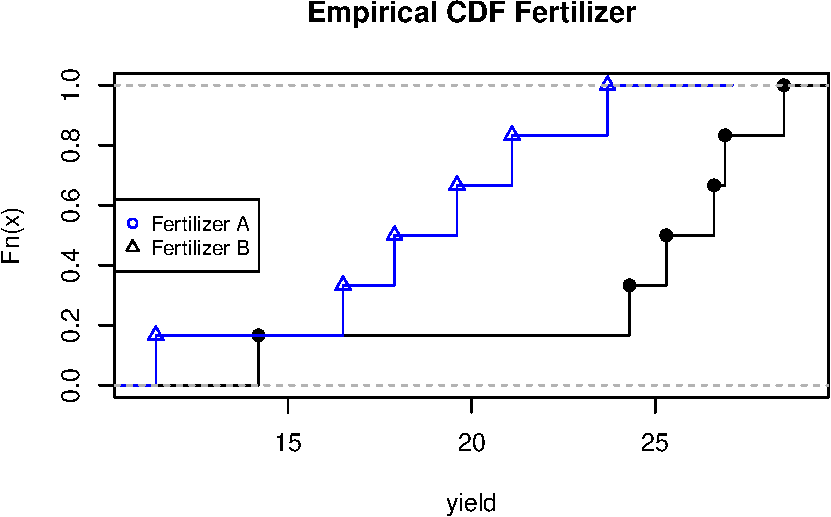
\includegraphics{class4slides-jan18_files/figure-beamer/unnamed-chunk-2-1.pdf}

\end{frame}

\begin{frame}[fragile]{Wheat Yield Study}

\begin{Shaded}
\begin{Highlighting}[]
\KeywordTok{summary}\NormalTok{(yA); }\KeywordTok{sd}\NormalTok{(yA);}\KeywordTok{quantile}\NormalTok{(yA,}\DataTypeTok{prob=}\KeywordTok{c}\NormalTok{(}\FloatTok{0.25}\NormalTok{,}\FloatTok{0.75}\NormalTok{))}
\end{Highlighting}
\end{Shaded}

\begin{verbatim}
##    Min. 1st Qu.  Median    Mean 3rd Qu.    Max. 
##   11.40   16.85   18.75   18.37   20.72   23.70
\end{verbatim}

\begin{verbatim}
## [1] 4.234934
\end{verbatim}

\begin{verbatim}
##    25%    75% 
## 16.850 20.725
\end{verbatim}

\begin{Shaded}
\begin{Highlighting}[]
\KeywordTok{summary}\NormalTok{(yB); }\KeywordTok{sd}\NormalTok{(yB); }\KeywordTok{quantile}\NormalTok{(yB,}\DataTypeTok{prob=}\KeywordTok{c}\NormalTok{(}\FloatTok{0.25}\NormalTok{,}\FloatTok{0.75}\NormalTok{))}
\end{Highlighting}
\end{Shaded}

\begin{verbatim}
##    Min. 1st Qu.  Median    Mean 3rd Qu.    Max. 
##   14.20   24.55   25.95   24.30   26.82   28.50
\end{verbatim}

\begin{verbatim}
## [1] 5.151699
\end{verbatim}

\begin{verbatim}
##    25%    75% 
## 24.550 26.825
\end{verbatim}

\end{frame}

\begin{frame}[fragile]{Results}

\begin{Shaded}
\begin{Highlighting}[]
\KeywordTok{mean}\NormalTok{(yA)-}\KeywordTok{mean}\NormalTok{(yB)}
\end{Highlighting}
\end{Shaded}

\begin{verbatim}
## [1] -5.933333
\end{verbatim}

\begin{itemize}
\tightlist
\item
  So there is a moderate/large difference in mean yield for these
  fertilizers.
\item
  Would you recommend B over A for future plantings?
\item
  Do you think these results generalize to a larger population?
\item
  Could the result be due to chance?
\end{itemize}

\end{frame}

\begin{frame}{Hypothesis Testing Via Randomization}

\begin{itemize}
\tightlist
\item
  Are the observed differences in yield due to fertilizer type?
\item
  Are the observed differences in yield due to plot-to-plot variation?
\end{itemize}

\end{frame}

\begin{frame}{Hypothesis Testing Via Randomization}

Hypothesis tests:

\begin{itemize}
\item
  \(H_0\) (null hypothesis): Fertilizer type does not affect yield.
\item
  \(H_1\) (alternative hypothesis): Fertilizer type does affect yield.
\item
  A statistical hypothesis evaluates the compatibility of \(H_0\) with
  the data
\end{itemize}

\end{frame}

\begin{frame}{Test Statistics and Null Distributions}

We can evaluate \(H_0\) by answering:

\begin{itemize}
\item
  Is a mean difference of -5.93 plausible/probable if H0 true?
\item
  Is a mean difference of -5.93 large compared to experimental noise?
\end{itemize}

\end{frame}

\begin{frame}{Test Statistics and Null Distributions}

\begin{itemize}
\item
  Compare \({\bar y}_a-{\bar y}_b\)=-5.93 (observed difference in the
  experiment) to values of \({\bar y}_a-{\bar y}_b\) that could have
  been observed if \(H_0\) were true.
\item
  Hypothetical values of \({\bar y}_a-{\bar y}_b\) that could have been
  observed under \(H_0\) are referred to as samples from the null
  distribution.
\end{itemize}

\end{frame}

\begin{frame}{Test Statistics and Null Distributions}

\begin{itemize}
\item
  \({\bar y}_a-{\bar y}_b\) is a function of the outcome of the
  experiment.
\item
  If a different experiment were performed then we would obtain a
  diffrent value of \({\bar y}_a-{\bar y}_b\).
\end{itemize}

\end{frame}

\begin{frame}{Test Statistics and Null Distributions}

\begin{itemize}
\tightlist
\item
  In this experiment we observed \({\bar y}_a-{\bar y}_b\)=-5.93.
\item
  If there was no difference between fertilizers then what other
  possible values of \({\bar y}_a-{\bar y}_b\) could have been observed?
\end{itemize}

\end{frame}

\begin{frame}{Experimental Procedure and Potential Outcomes}

The cards were shuffled and we were dealt B, R, B, R, \ldots{}

\begin{table}[]
\centering
\label{my-label}
\begin{tabular}{|l|l|l|l|l|l|}
\hline
B  & A  & B  & A  & B   & B  \\ \hline
B  & A  & A  & A  & B  & A  \\ \hline
\end{tabular}
\end{table}

Under this treatment assignment we oberved the yields:

\begin{table}[]
\centering
\label{my-label}
\begin{tabular}{|l|l|l|l|l|l|}
\hline
B 26.9 & A 11.4 & B 26.6 & A 23.7 & B 25.3  & B 28.5 \\ \hline
B 14.2 & A 17.9 & A 16.5 & A 21.1 & B 24.3 & A 19.6 \\ \hline
\end{tabular}
\end{table}

\end{frame}

\begin{frame}{Experimental Procedure and Potential Outcomes}

Another potential treatment assignment under \(H_0\) is:

\begin{table}[]
\centering
\label{my-label}
\begin{tabular}{|l|l|l|l|l|l|}
\hline
B  & A  & B  & B  & A   & A  \\ \hline
A  & B  & B  & A  & A  & B  \\ \hline
\end{tabular}
\end{table}

The yields obtained under this assignment are:

\begin{table}[]
\centering
\label{my-label}
\begin{tabular}{|l|l|l|l|l|l|}
\hline
B 26.9 & A 11.4 & B 26.6 & B 23.7 & A 25.3  & A 28.5 \\ \hline
A 14.2 & B 17.9 & B 16.5 & A 21.1 & A 24.3 & B 19.6 \\ \hline
\end{tabular}
\end{table}

This data could occur if the experiment were run again.

\end{frame}

\begin{frame}[fragile]{Experimental Procedure and Potential Outcomes}

\begin{itemize}
\tightlist
\item
  Under this hypothetical assignment the mean difference is:
\end{itemize}

\begin{Shaded}
\begin{Highlighting}[]
\NormalTok{yA <-}\StringTok{ }\KeywordTok{c}\NormalTok{(}\FloatTok{11.4}\NormalTok{,}\FloatTok{25.3}\NormalTok{,}\FloatTok{28.5}\NormalTok{,}\FloatTok{14.2}\NormalTok{,}\FloatTok{21.1}\NormalTok{,}\FloatTok{24.3}\NormalTok{)}
\NormalTok{yB <-}\StringTok{ }\KeywordTok{c}\NormalTok{(}\FloatTok{26.9}\NormalTok{,}\FloatTok{26.6}\NormalTok{,}\FloatTok{23.7}\NormalTok{,}\FloatTok{17.9}\NormalTok{,}\FloatTok{16.5}\NormalTok{,}\FloatTok{19.6}\NormalTok{)}
\KeywordTok{mean}\NormalTok{(yA-yB)}
\end{Highlighting}
\end{Shaded}

\begin{verbatim}
## [1] -1.066667
\end{verbatim}

This represents an outcome of the experiment in a universe where:

\begin{enumerate}
\def\labelenumi{\arabic{enumi}.}
\item
  The treatment assignment is B, A, B, B, A, A, A, B, B, A, A, B
\item
  \(H_0\) is true (i.e., \(\mu_A=\mu_B\), where \(\mu_A,\mu_B\) are the
  mean yields of fertilizers A and B).
\end{enumerate}

\end{frame}

\begin{frame}{The Null distribution}

\begin{itemize}
\tightlist
\item
  What potential outcomes \textbf{could} we see if \(H_0\) is true?
\item
  Compute \({\bar y}_a-{\bar y}_b\) for each possible treatment
  assignment.
\end{itemize}

\end{frame}

\begin{frame}{The Null Distribution}

\begin{itemize}
\tightlist
\item
  For each treatment assignment compute
  \[\delta_i={\bar y_a}-{\bar y_b}, i=1,2,\ldots,924.\]
\item
  \(\left\{\delta_1, \delta_2, \ldots, \delta_{924}\right\}\) enumerates
  all pre-randomisation outcomes assuming no treatment effect.
\item
  Since each treatment assignment is equally likely under the null
  distribution, a probability distribution of experimental results if
  \(H_0\) is true can be described as
\end{itemize}

\[\begin{aligned} 
{\hat F}(y) &= \frac{\#(\delta_i \le y)}{924} \\
            &= \frac{\sum_{k=1}^{{\binom{12}{6}}}I({\delta_k \le y})}{\binom{12}{6}}
\end{aligned}\]

This is called the randomisation distribution.

\end{frame}

\begin{frame}{Randomization Distribution}

\begin{itemize}
\item
  The yield is not random since the plots were not chosen randomly.
\item
  Their assignment to treatments is random.
\item
  The basis for building a probability distribution for
  \(\bar{y}_a - \bar{y}_b\) comes from the randomization of fertilizers
  to plots.
\end{itemize}

\end{frame}

\begin{frame}{Randomization Distribution}

\begin{itemize}
\item
  This randomization results in 6 plots getting fertilizer A and the
  remaining 6 plots receiving fertilizer B.
\item
  This is one of \({12 \choose 6} = 924\) equally likely randomizations
  that could have occured.
\end{itemize}

\end{frame}

\begin{frame}{Experimental Procedure and Potential Outcomes}

This represents an outcome of the experiment in a universe where:

\begin{enumerate}
\def\labelenumi{\arabic{enumi}.}
\item
  \(H_0\) is true.
\item
  The yield will be the same regardless of which fertilizer a plot
  received.
\end{enumerate}

For example a plot that had a yield of 26.9 given fertilizer B would
have the same yield if the plot received fertilizer A if \(H_0\) is
true.

\end{frame}

\begin{frame}[fragile]{R Code for Randomization Distribution}

\begin{Shaded}
\begin{Highlighting}[]
\NormalTok{yA <-}\StringTok{ }\KeywordTok{c}\NormalTok{(}\FloatTok{11.4}\NormalTok{,}\FloatTok{23.7}\NormalTok{,}\FloatTok{17.9}\NormalTok{,}\FloatTok{16.5}\NormalTok{,}\FloatTok{21.1}\NormalTok{,}\FloatTok{19.6}\NormalTok{);yB <-}\StringTok{ }\KeywordTok{c}\NormalTok{(}\FloatTok{26.9}\NormalTok{,}\FloatTok{26.6}\NormalTok{,}\FloatTok{25.3}\NormalTok{,}\FloatTok{28.5}\NormalTok{,}\FloatTok{14.2}\NormalTok{,}\FloatTok{24.3}\NormalTok{)}
\NormalTok{fert <-}\StringTok{ }\KeywordTok{c}\NormalTok{(yA,yB); N <-}\StringTok{ }\KeywordTok{choose}\NormalTok{(}\DecValTok{12}\NormalTok{,}\DecValTok{6}\NormalTok{)}
\NormalTok{res <-}\StringTok{ }\KeywordTok{numeric}\NormalTok{(N) }\CommentTok{# store the results}
\NormalTok{index <-}\KeywordTok{combn}\NormalTok{(}\DecValTok{1}\NormalTok{:}\DecValTok{12}\NormalTok{,}\DecValTok{6}\NormalTok{) }\CommentTok{#Generate N treatment assignments}
\NormalTok{for (i in }\DecValTok{1}\NormalTok{:N)}
\NormalTok{\{res[i] <-}\StringTok{ }\KeywordTok{mean}\NormalTok{(fert[index[,i]])-}\KeywordTok{mean}\NormalTok{(fert[-index[,i]])\}}
\NormalTok{index[,}\DecValTok{1}\NormalTok{:}\DecValTok{2}\NormalTok{] }\CommentTok{#output first two randomizations}
\end{Highlighting}
\end{Shaded}

\begin{verbatim}
##      [,1] [,2]
## [1,]    1    1
## [2,]    2    2
## [3,]    3    3
## [4,]    4    4
## [5,]    5    5
## [6,]    6    7
\end{verbatim}

\begin{Shaded}
\begin{Highlighting}[]
\NormalTok{res[}\DecValTok{1}\NormalTok{:}\DecValTok{2}\NormalTok{] }\CommentTok{#output first two mean diffs}
\end{Highlighting}
\end{Shaded}

\begin{verbatim}
## [1] -5.933333 -3.500000
\end{verbatim}

\end{frame}

\begin{frame}{Randomization Distribution}

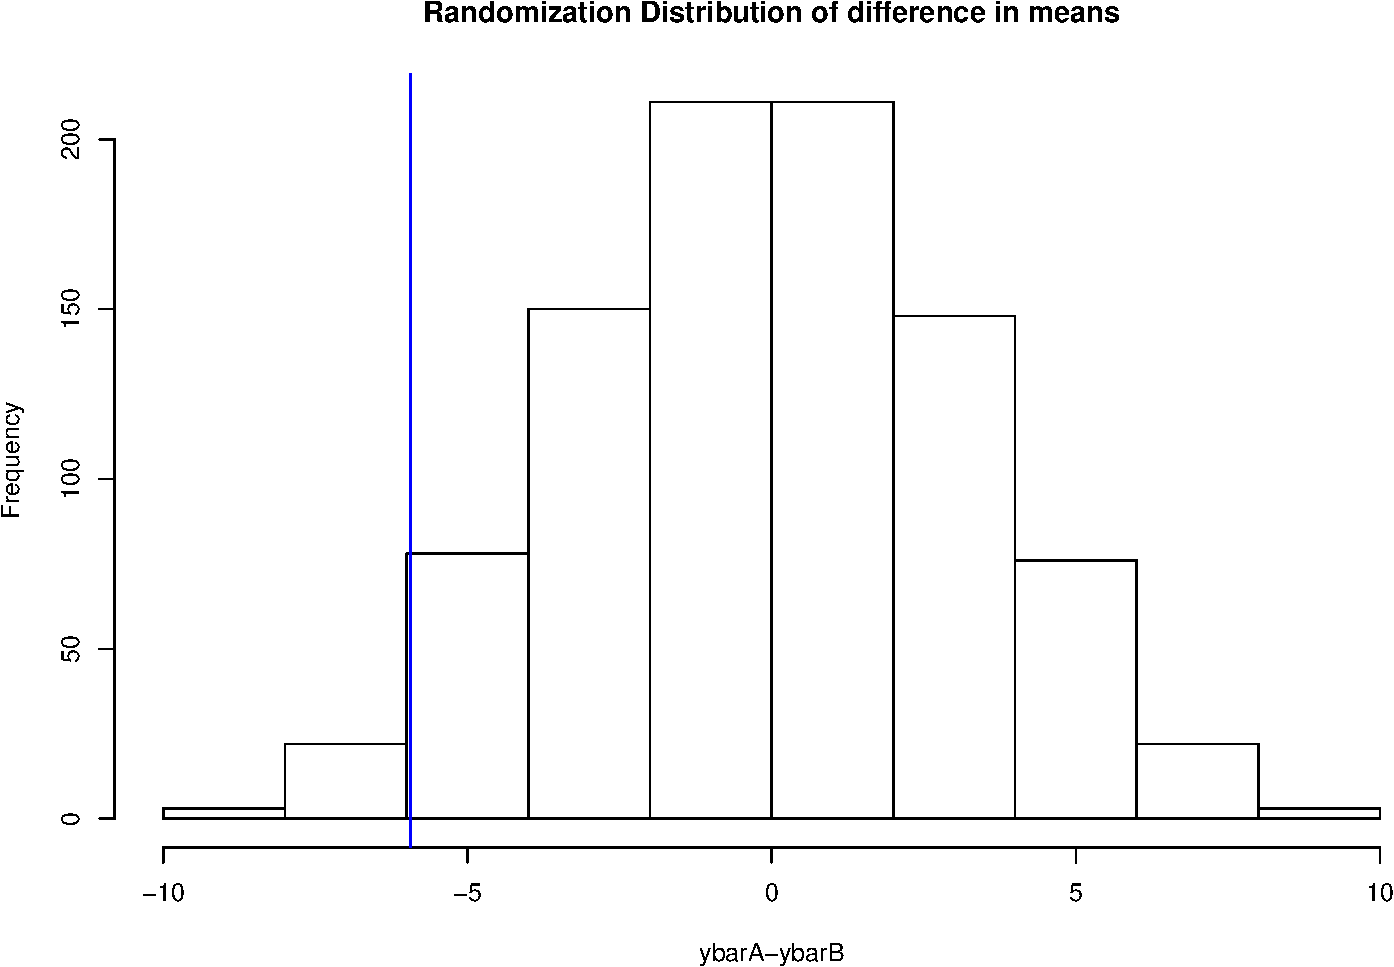
\includegraphics{class4slides-jan18_files/figure-beamer/unnamed-chunk-7-1.pdf}

\end{frame}

\begin{frame}{Hypothesis Testing}

\begin{itemize}
\tightlist
\item
  Is there any contradiction between \(H_0\) and the observed data?
\item
  A \textbf{P-value} is the probability, under the null hypothesis of
  obtaining a more extreme than the observed result.
\end{itemize}

\[ \text{P-value}=P\left(\delta \le -5.93 \right)={\hat F}(-5.93)\]

\begin{itemize}
\item
  A small P-value implies evidence \textbf{against} null hypothesis.
\item
  If the P-value is large does this imply that the null is true?
\end{itemize}

\end{frame}

\begin{frame}{Randomization Test}

\begin{itemize}
\item
  Assume \(H_0\) is true.
\item
  Calculate the difference in means for every possible way to split the
  data into two samples of size 6.
\item
  This would result in \({{12}\choose{6}}=924\) differences.
\item
  Calculate the probability of observing a value as extreme of more
  extreme than the observed value of the test statistic
  (\emph{P-value}).
\item
  If the P-value is small then there are two possible explanations:
\end{itemize}

\begin{enumerate}
\def\labelenumi{\arabic{enumi}.}
\item
  An unlikely value of the statistic has occurred, or
\item
  The assumption that \(H_0\) is true is incorrect.
\end{enumerate}

\begin{itemize}
\tightlist
\item
  If the P-value is large then the hypothesis test is inconclusive.
\end{itemize}

\end{frame}

\begin{frame}[fragile]{Computing the P-value}

The observed value of the test statistic is -5.93. So, the p-value is

\begin{Shaded}
\begin{Highlighting}[]
\CommentTok{# of times values from the mean randomization distribution }
\CommentTok{# less than observed value}
\KeywordTok{sum}\NormalTok{(res<=observed) }
\end{Highlighting}
\end{Shaded}

\begin{verbatim}
## [1] 26
\end{verbatim}

\begin{Shaded}
\begin{Highlighting}[]
\NormalTok{N }\CommentTok{# Number of randomizations}
\end{Highlighting}
\end{Shaded}

\begin{verbatim}
## [1] 924
\end{verbatim}

\begin{Shaded}
\begin{Highlighting}[]
\NormalTok{pval <-}\StringTok{ }\KeywordTok{sum}\NormalTok{(res<=observed)/N }\CommentTok{# Randomization p value}
\KeywordTok{round}\NormalTok{(pval,}\DecValTok{2}\NormalTok{)}
\end{Highlighting}
\end{Shaded}

\begin{verbatim}
## [1] 0.03
\end{verbatim}

\end{frame}

\begin{frame}{Interpretation of P-value}

\begin{itemize}
\item
  A p-value of 0.03 can be interpreted as: assume there is no difference
  in yield between fertilizers A and B then the proportion of
  randomizations that would produce an observed mean difference between
  A and B of at most -5.93 is 0.03.
\item
  In other words, under the assumption that there is no difference
  between A and B only 3\% of randomizations would produce an extreme or
  more extreme difference than the observed mean difference.
\item
  Therefore it's unlikely (if we consider 3\% unlikely) that an observed
  mean difference as extreme or more extreme than -5.93 would be
  observed if \(\mu_A=\mu_B\).
\end{itemize}

\end{frame}

\begin{frame}{Two-Sided Randomization P value}

\begin{itemize}
\item
  If we are using a two-sided alternative then how do we calculate a
  p-value?
\item
  The randomization distribution may not be symmetric so there is no
  justifcation for simply doubling the probability in one tail.
\end{itemize}

Let

\[{\bar t}=\left(1/{N \choose N_A}\right) {\sum_{i=1}^{N \choose N_A} t_i}\]

be the mean of the randomization distribution then we can define the
two-sided p-value as

\[P(\left|T-{\bar t}\right| \ge \left|t^{*}-{\bar t}\right||H_0) = \sum_{i=1}^{N \choose N_A} \frac{I(\left|t_i-{\bar t}\right| \ge \left|t^{*}-{\bar t}\right|)}{{N \choose N_A}},\]

The probability of obtaining an observed value of the test statistic as
far, or farther, from the mean of the randomization distribution.

\end{frame}

\begin{frame}[fragile]{Two-Sided Randomization P value}

\begin{Shaded}
\begin{Highlighting}[]
\NormalTok{yA <-}\StringTok{ }\KeywordTok{c}\NormalTok{(}\FloatTok{11.4}\NormalTok{,}\FloatTok{23.7}\NormalTok{,}\FloatTok{17.9}\NormalTok{,}\FloatTok{16.5}\NormalTok{,}\FloatTok{21.1}\NormalTok{,}\FloatTok{19.6}\NormalTok{)}
\NormalTok{yB <-}\StringTok{ }\KeywordTok{c}\NormalTok{(}\FloatTok{26.9}\NormalTok{,}\FloatTok{26.6}\NormalTok{,}\FloatTok{25.3}\NormalTok{,}\FloatTok{28.5}\NormalTok{,}\FloatTok{14.2}\NormalTok{,}\FloatTok{24.3}\NormalTok{)}
\NormalTok{fert <-}\StringTok{ }\KeywordTok{c}\NormalTok{(yA,yB) }\CommentTok{#pool data}
\NormalTok{N <-}\StringTok{ }\KeywordTok{choose}\NormalTok{(}\DecValTok{12}\NormalTok{,}\DecValTok{6}\NormalTok{)}
\NormalTok{res <-}\StringTok{ }\KeywordTok{numeric}\NormalTok{(N) }\CommentTok{# store the results}
\NormalTok{index <-}\KeywordTok{combn}\NormalTok{(}\DecValTok{1}\NormalTok{:}\DecValTok{12}\NormalTok{,}\DecValTok{6}\NormalTok{)}
\NormalTok{for (i in }\DecValTok{1}\NormalTok{:N)}
\NormalTok{\{}
  \NormalTok{res[i] <-}\StringTok{ }\KeywordTok{mean}\NormalTok{(fert[index[,i]])-}\KeywordTok{mean}\NormalTok{(fert[-index[,i]])}
\NormalTok{\}}
\NormalTok{tbar <-}\StringTok{ }\KeywordTok{mean}\NormalTok{(res)}
\NormalTok{pval <-}\StringTok{ }\KeywordTok{sum}\NormalTok{(}\KeywordTok{abs}\NormalTok{(res-tbar)>=}\KeywordTok{abs}\NormalTok{(observed-tbar))/N}
\KeywordTok{round}\NormalTok{(pval,}\DecValTok{2}\NormalTok{)}
\end{Highlighting}
\end{Shaded}

\begin{verbatim}
## [1] 0.06
\end{verbatim}

\end{frame}

\begin{frame}{Randomization Test}

\begin{itemize}
\item
  We could calculate the difference in means for every possible way to
  split the data into two samples of size 6.
\item
  This would result in \({12 \choose 6} =924\) differences.
\item
  If there were 30 observations split evenly into two groups then there
  are \({30 \choose 15}=155,117, 520\) differences.
\item
  So unless the sample sizes are small these exhaustive calculations are
  not practical.
\end{itemize}

\end{frame}

\begin{frame}{Randomization Test}

Instead we can create a permutation resample (Monte Carlo Sampling).

\begin{enumerate}
\def\labelenumi{\arabic{enumi}.}
\item
  Draw 6 observations from the pooled data without replacement. (fert A)
\item
  The remaining 6 observations will be the second sample (fert B)
\item
  Calculate the difference in means of the two samples
\item
  Repeat 1-3 at least 250000 times.
\item
  P-value is the fraction of times the random statistics exceeds the
  original statistic.
\end{enumerate}

\end{frame}

\begin{frame}{Estimate P-value via Monte Carlo Sampling}

If \(M\) test statistics, \(t_i\), \(i=1,...,M\) are randomly sampled
from the permutation distribution, a one-sided Monte Carlo p value for a
test of \(H_0: \mu_T=0\) versus \(H_1: \mu_T > 0\) is

\[ {\hat p} = \frac {1+\sum_{i=1}^M I(t_i \ge t^{*})}{M+1}.\]

Including the observed value \(t^{*}\) there are \(M+1\) test
statistics.

\end{frame}

\begin{frame}[fragile]{Estimate P-value via Monte Carlo Sampling}

\begin{Shaded}
\begin{Highlighting}[]
\NormalTok{N <-}\StringTok{ }\DecValTok{250000} \CommentTok{# number of times to repeat this process}
\NormalTok{result <-}\StringTok{ }\KeywordTok{numeric}\NormalTok{(N) }\CommentTok{# space to save random diffs.}
\NormalTok{for (i in }\DecValTok{1}\NormalTok{:N)}
\NormalTok{\{ }\CommentTok{#sample of size 6, from 1 to 12, without replacement}
  \NormalTok{index <-}\StringTok{ }\KeywordTok{sample}\NormalTok{(}\DecValTok{12}\NormalTok{,}\DataTypeTok{size=}\DecValTok{6}\NormalTok{,}\DataTypeTok{replace=}\NormalTok{F)}
  \NormalTok{result[i] <-}\StringTok{ }\KeywordTok{mean}\NormalTok{(fert[index])-}\KeywordTok{mean}\NormalTok{(fert[-index])}
\NormalTok{\}}

\CommentTok{#store observed mean difference}
\NormalTok{observed <-}\StringTok{ }\KeywordTok{mean}\NormalTok{(yA)-}\KeywordTok{mean}\NormalTok{(yB)}

\CommentTok{#P-value - mean - results will vary}
\NormalTok{pval <-}\StringTok{ }\NormalTok{(}\KeywordTok{sum}\NormalTok{(result <=}\StringTok{ }\NormalTok{observed)+}\DecValTok{1}\NormalTok{)/(N}\DecValTok{+1}\NormalTok{)}
\KeywordTok{round}\NormalTok{(pval,}\DecValTok{4}\NormalTok{)}
\end{Highlighting}
\end{Shaded}

\begin{verbatim}
## [1] 0.0279
\end{verbatim}

\end{frame}

\begin{frame}{Basic Decision Theory}

\begin{table}[]
\centering
\label{my-label}
\begin{tabular}{l|l|l}
          & $H_0$ True      & $H_0$ False      \\
          \hline
Accept $H_0$ & correct      & type II error \\
\hline
Reject $H_0$ & type I error & correct      
\end{tabular}
\end{table}

\[\text{P-value}=P\left(\text{test statistic} \ge \text{observed value of test statistic} \right) \]

\[\begin{aligned} 
\alpha&=P\left(\text{type I error}\right)  \\
\beta &=P\left(\text{type II error}\right) \\
1-\beta &=\text{power}
\end{aligned}\]

\end{frame}

\begin{frame}{The Randomization P-value}

\begin{itemize}
\item
  An achievable P-value of the randomization test must be a multiple of
  \(\frac{k}{\binom{12}{6}} = \frac{k}{924}\), where
  \(k=1,2,\ldots,924\).
\item
  If we choose a significance level of \(\alpha=\frac{k}{924}\) that is
  one of the achievable P-values then
  \(P\left(\text{type I error}\right)=\alpha\).
\item
  The randomization test is an exact test.
\item
  If \(\alpha\) is not chosen to be one of the achievable P-values but
  \(\alpha=\frac{k}{924}\) is the largest acheivable P-value less than
  \(\alpha\) then \(P\left(\text{type I error}\right) < \alpha\).
\end{itemize}

\end{frame}

\begin{frame}{Choosing a Test Statistic}

A test statistic should be able to differentiate between \(H_0\) and
\(H_a\) in ways that are scientifically relevant.

\end{frame}

\begin{frame}{Other Test Statistics}

\begin{itemize}
\item
  Other test statistics could be used instead of
  \(T={\bar Y}_A-{\bar Y}_B\) to measure the effectiveness of fertilizer
  A.
\item
  The difference in group medians
\end{itemize}

\[median(Y_A)-median(Y_B) \]

or trimmed means are examples of other test statistics.

\end{frame}

\begin{frame}[fragile]{Other Test Statistics}

The randomiztion distribution of the difference in group medians can be
obtained by modifying the R code used for the difference in group means.

\begin{Shaded}
\begin{Highlighting}[]
\NormalTok{fert <-}\StringTok{ }\KeywordTok{c}\NormalTok{(yA,yB) }\CommentTok{#pool data}
\NormalTok{N <-}\StringTok{ }\KeywordTok{choose}\NormalTok{(}\DecValTok{12}\NormalTok{,}\DecValTok{6}\NormalTok{)}
\NormalTok{res <-}\StringTok{ }\KeywordTok{numeric}\NormalTok{(N) }\CommentTok{# store the results}
\NormalTok{index <-}\KeywordTok{combn}\NormalTok{(}\DecValTok{1}\NormalTok{:}\DecValTok{12}\NormalTok{,}\DecValTok{6}\NormalTok{) }\CommentTok{# Generate N treatment assignments}
\NormalTok{for (i in }\DecValTok{1}\NormalTok{:N)}
\NormalTok{\{}
  \NormalTok{res[i] <-}\StringTok{ }\KeywordTok{median}\NormalTok{(fert[index[,i]])-}\KeywordTok{median}\NormalTok{(fert[-index[,i]])}
\NormalTok{\}}
\end{Highlighting}
\end{Shaded}

\end{frame}

\begin{frame}{Other Test Statistics}

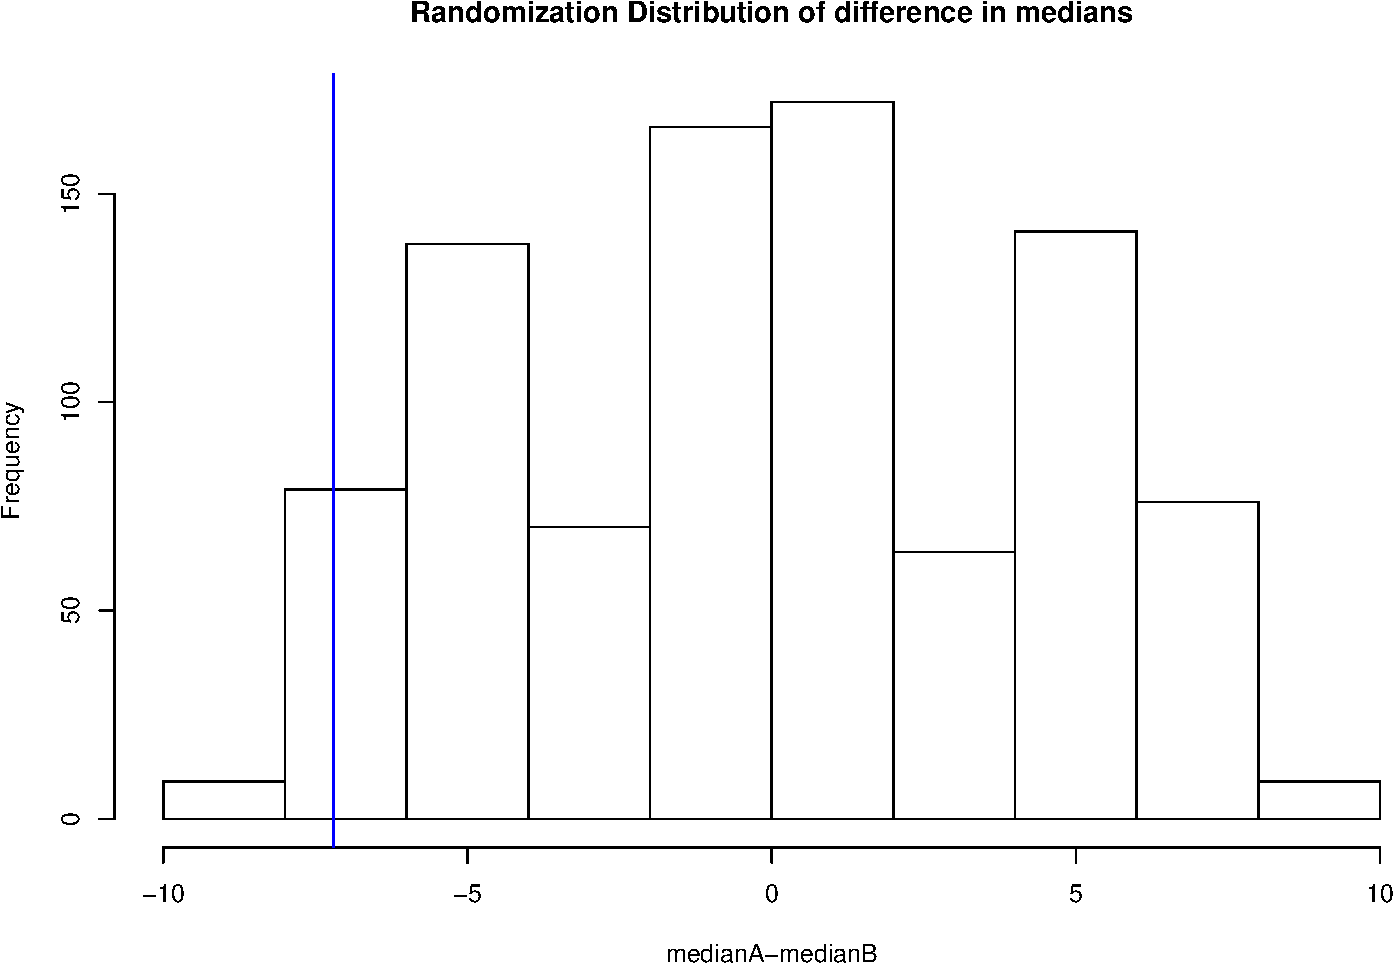
\includegraphics{class4slides-jan18_files/figure-beamer/unnamed-chunk-12-1.pdf}

\end{frame}

\begin{frame}[fragile]{Other Test Statistics}

The p-value of the randomization test can be calculated

\begin{Shaded}
\begin{Highlighting}[]
\CommentTok{# of times values from the median randomization }
\CommentTok{# distribution less than observed value}
\KeywordTok{sum}\NormalTok{(res<=observed) }
\end{Highlighting}
\end{Shaded}

\begin{verbatim}
## [1] 36
\end{verbatim}

\begin{Shaded}
\begin{Highlighting}[]
\NormalTok{N }\CommentTok{# Number of randomizations}
\end{Highlighting}
\end{Shaded}

\begin{verbatim}
## [1] 924
\end{verbatim}

\begin{Shaded}
\begin{Highlighting}[]
\NormalTok{pval <-}\StringTok{ }\KeywordTok{sum}\NormalTok{(res<=observed)/N }\CommentTok{# Randomization p value}
\KeywordTok{round}\NormalTok{(pval,}\DecValTok{2}\NormalTok{)}
\end{Highlighting}
\end{Shaded}

\begin{verbatim}
## [1] 0.04
\end{verbatim}

\end{frame}

\begin{frame}{The two-sample t-test}

If the two wheat yield samples are independent random samples from a
normal distribution with means \(\mu_A\) and \(\mu_B\) but the same
variance then the statistic

\[ {\bar y}_A - {\bar y}_b \sim N\left(\mu_A-\mu_B,\sigma^2(1/n_A+1/n_B) \right).\]

So,

\[ \frac {{\bar y}_A - {\bar y}_b- \delta}{\sigma \sqrt{(1/n_A+1/n_B)}} \sim N(0,1),\]

where \(\delta=\mu_A-\mu_B\).

If we substitute

\[S^2=\frac{\sum_{i=1}^{n_A}(y_{iA}-{\bar y}_A)+\sum_{i=1}^{n_B}(y_{iB}-{\bar y}_B)}{n_A+n_B-2}\]

for \(\sigma^2\) then

\[ \frac {{\bar y}_A - {\bar y}_b - \delta}{s \sqrt{(1/n_A+1/n_B)}} \sim t_{n_A+n_B-2},\]

is called the two sample t-statistic.

\end{frame}

\begin{frame}[fragile]{The two-sample t-test}

In the wheat yield example \(H_0:\mu_A=\mu_B\) and suppose that
\(H_1: \mu_A < \mu_B.\) The p-value of the test is obtained by
calculating the observed value of the two sample t-statistic under
\(H_0\).

\[ t^{*}= \frac {{\bar y}_A - {\bar y}_b}{s \sqrt{(1/n_A+1/n_B)}} = \frac {18.37 - 24.3}{4.72 \sqrt{(1/6+1/6)}}=-2.18\]

The p-value is \(P(t_{18}<-2.18)=\) 0.03.

The calculation was done in R.

\begin{Shaded}
\begin{Highlighting}[]
\NormalTok{s <-}\StringTok{ }\KeywordTok{sqrt}\NormalTok{((}\DecValTok{5}\NormalTok{*}\KeywordTok{var}\NormalTok{(yA)+}\DecValTok{5}\NormalTok{*}\KeywordTok{var}\NormalTok{(yB))/}\DecValTok{10}\NormalTok{)}
\NormalTok{tstar <-}\StringTok{ }\NormalTok{(}\KeywordTok{mean}\NormalTok{(yA)-}\KeywordTok{mean}\NormalTok{(yB))/(s*}\KeywordTok{sqrt}\NormalTok{(}\DecValTok{1}\NormalTok{/}\DecValTok{6+1}\NormalTok{/}\DecValTok{6}\NormalTok{)); }\KeywordTok{round}\NormalTok{(tstar,}\DecValTok{2}\NormalTok{)}
\end{Highlighting}
\end{Shaded}

\begin{verbatim}
## [1] -2.18
\end{verbatim}

\begin{Shaded}
\begin{Highlighting}[]
\NormalTok{pval <-}\StringTok{ }\KeywordTok{pt}\NormalTok{(tstar,}\DecValTok{10}\NormalTok{); }\KeywordTok{round}\NormalTok{(pval,}\DecValTok{5}\NormalTok{)}
\end{Highlighting}
\end{Shaded}

\begin{verbatim}
## [1] 0.02715
\end{verbatim}

\end{frame}

\begin{frame}[fragile]{The two-sample t-test}

In R the command to run a two-sample t-test is \texttt{t.test()}.

\begin{Shaded}
\begin{Highlighting}[]
\KeywordTok{t.test}\NormalTok{(yA,yB,}\DataTypeTok{var.equal =} \OtherTok{TRUE}\NormalTok{,}\DataTypeTok{alternative =} \StringTok{"less"}\NormalTok{)}
\end{Highlighting}
\end{Shaded}

\begin{verbatim}
## 
##  Two Sample t-test
## 
## data:  yA and yB
## t = -2.1793, df = 10, p-value = 0.02715
## alternative hypothesis: true difference in means is less than 0
## 95 percent confidence interval:
##        -Inf -0.9987621
## sample estimates:
## mean of x mean of y 
##  18.36667  24.30000
\end{verbatim}

\end{frame}

\begin{frame}[fragile]{The two-sample t-test}

The assumption of normality can be checked using normal quantile plots,
although the t-test is robust against non-normality.

\begin{Shaded}
\begin{Highlighting}[]
\KeywordTok{qqnorm}\NormalTok{(yA,}\DataTypeTok{main =} \StringTok{"Fertilizer A"}\NormalTok{);}\KeywordTok{qqline}\NormalTok{(yA)}
\end{Highlighting}
\end{Shaded}

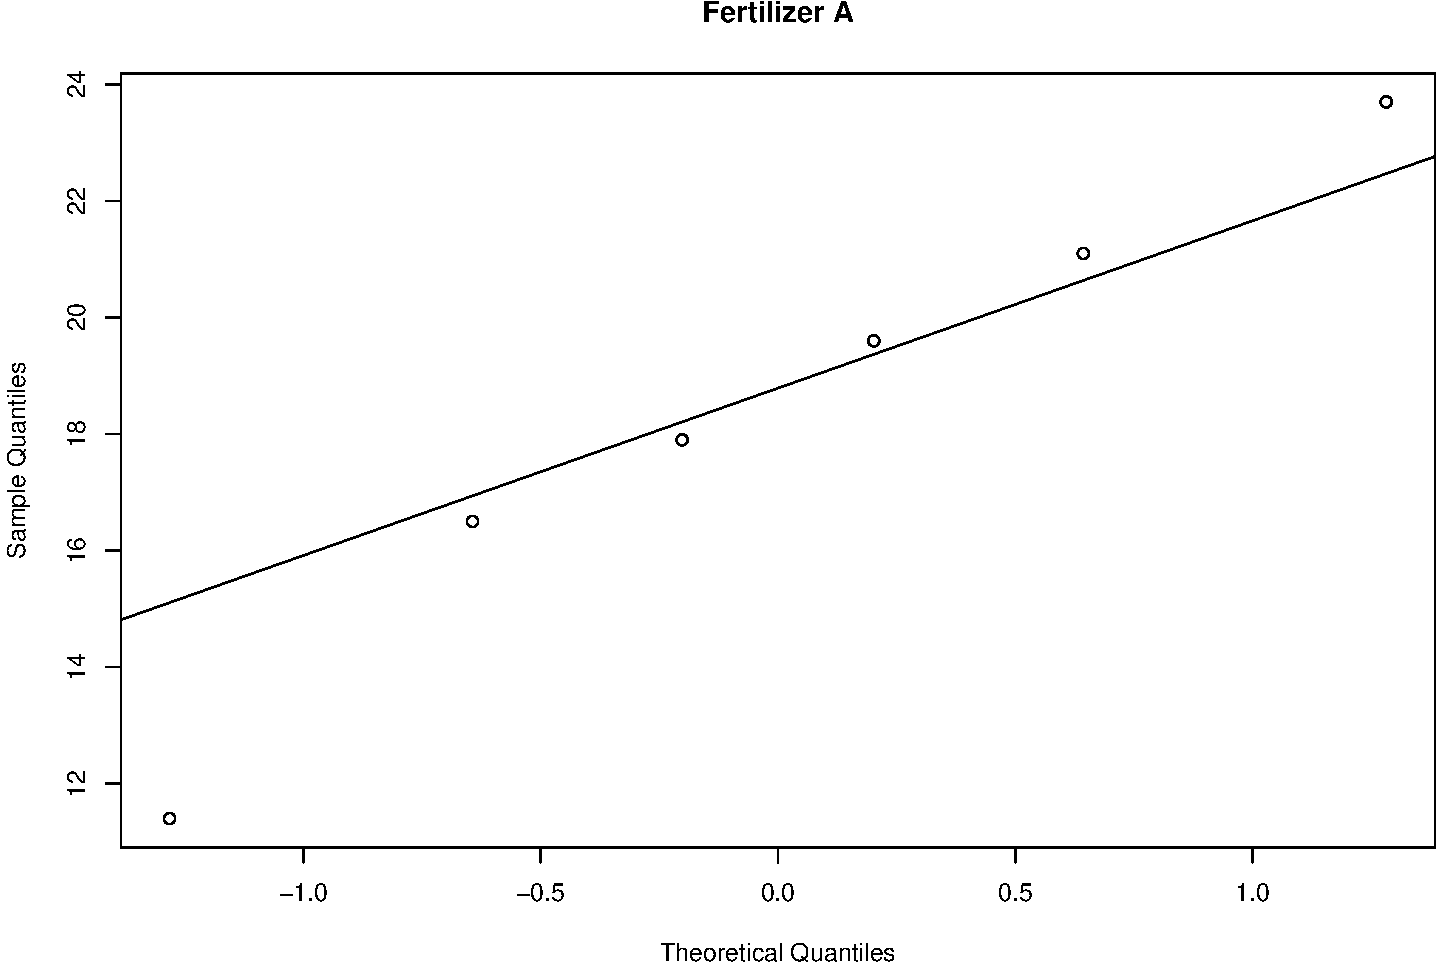
\includegraphics{class4slides-jan18_files/figure-beamer/unnamed-chunk-16-1.pdf}

\end{frame}

\begin{frame}[fragile]{The two-sample t-test}

\begin{Shaded}
\begin{Highlighting}[]
\KeywordTok{qqnorm}\NormalTok{(yB,}\DataTypeTok{main =} \StringTok{"Fertilizer B"}\NormalTok{);}\KeywordTok{qqline}\NormalTok{(yB)}
\end{Highlighting}
\end{Shaded}

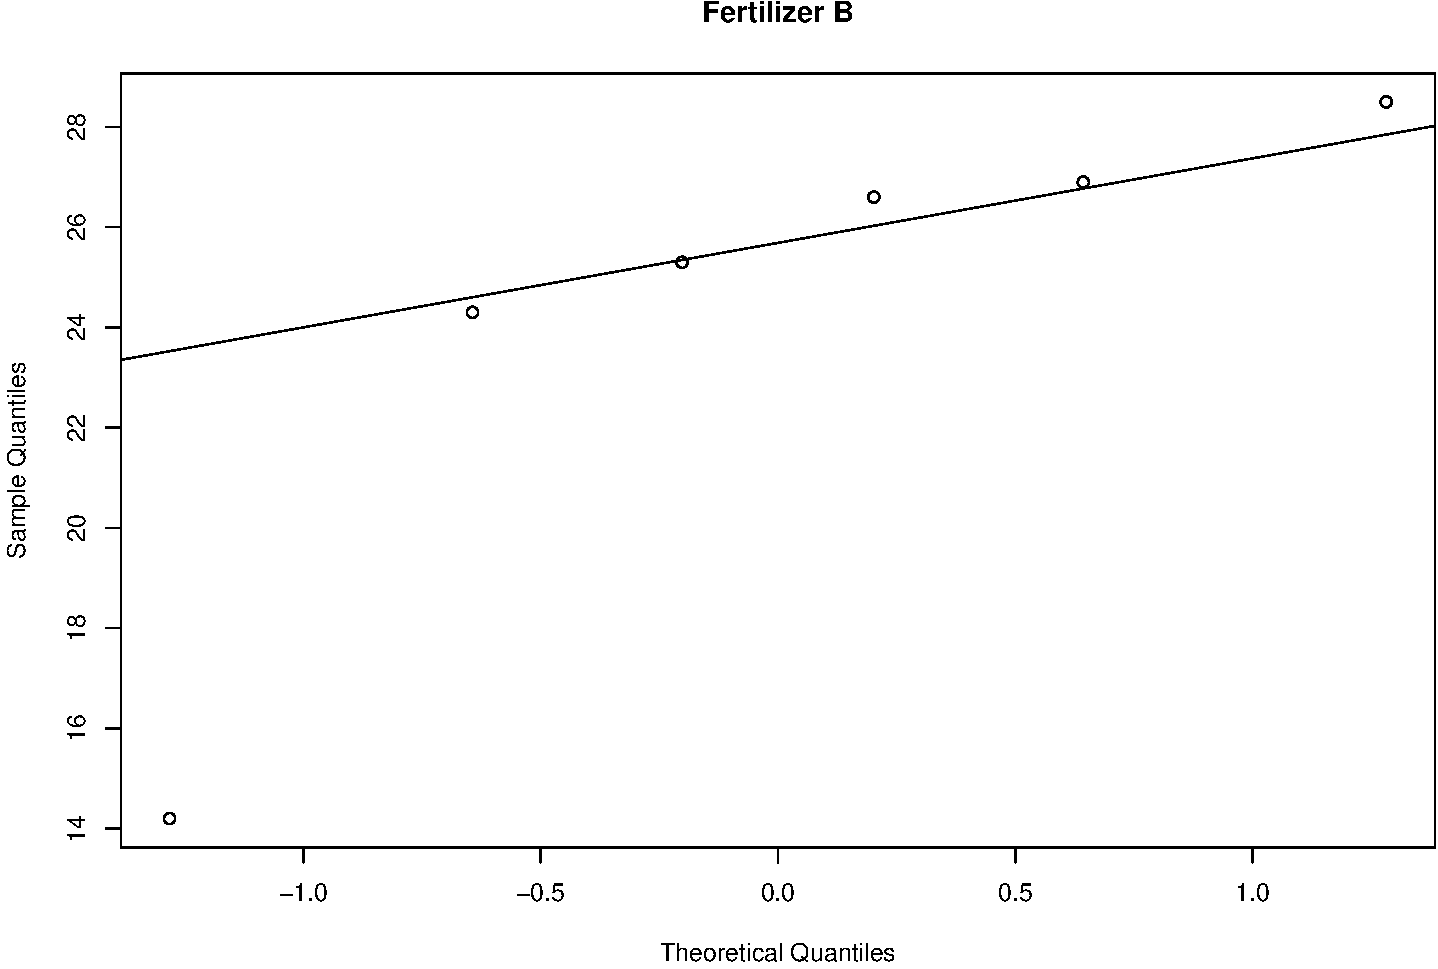
\includegraphics{class4slides-jan18_files/figure-beamer/unnamed-chunk-17-1.pdf}

\end{frame}

\begin{frame}{Two-Sample t-test versus Randomization Test}

\begin{itemize}
\item
  The p-value from the randomization test and the p-value from
  two-sample t-test are almost identical.
\item
  The randomization test does not depend on normality or independence.
\end{itemize}

\end{frame}

\begin{frame}{Two-Sample t-test versus Randomization Test}

\begin{itemize}
\item
  The randomization test does depend on Fisher's concept that after
  randomization, if the null hypothesis is true, the two results
  obtained from each particular plot will be exchangeable.
\item
  The randomization test tells you what you could say if exchangeability
  were true.
\end{itemize}

\end{frame}

\begin{frame}{Paired Comparisons}

\begin{itemize}
\item
  Increase precision by making comparisons within matched pairs of
  experimental material.
\item
  Randomize within a pair.
\end{itemize}

\end{frame}

\begin{frame}{Boy's Shoe Experiment}

\begin{itemize}
\item
  Two materials to make boy's shoes, A and B, are tested to evaluate if
  B is more sturdy compared to A.
\item
  During the experimental test some boys scuffed their shoes more than
  others.
\item
  Each boy's two shoes were subjected to the same treatment by having
  each boy wear both materials.
\item
  Working with 10 differences B-A most of the boy-to-boy variation could
  be eliminated.
\item
  Called a randomized paired comparison design.
\end{itemize}

\end{frame}

\begin{frame}{Boy's Shoe Experiment}

\begin{itemize}
\item
  Toss a coin to randomize material to L/R foot of a boy.
\item
  Head: Material A used on right foot.
\item
  Null hypothesis: amount of wear associated with material A and B are
  the same.
\item
  So labelling given to a pair of results only affects the sign of the
  difference.
\end{itemize}

\end{frame}

\begin{frame}[fragile]{Randomized paired comparison}

\begin{Shaded}
\begin{Highlighting}[]
\KeywordTok{library}\NormalTok{(BHH2)}
\KeywordTok{data}\NormalTok{(shoes.data)}
\NormalTok{shoes.data}
\end{Highlighting}
\end{Shaded}

\begin{verbatim}
##    boy matA sideA matB sideB
## 1    1 13.2     L 14.0     R
## 2    2  8.2     L  8.8     R
## 3    3 10.9     R 11.2     L
## 4    4 14.3     L 14.2     R
## 5    5 10.7     R 11.8     L
## 6    6  6.6     L  6.4     R
## 7    7  9.5     L  9.8     R
## 8    8 10.8     L 11.3     R
## 9    9  8.8     R  9.3     L
## 10  10 13.3     L 13.6     R
\end{verbatim}

\end{frame}

\begin{frame}[fragile]{Randomized paired comparison}

\begin{Shaded}
\begin{Highlighting}[]
\KeywordTok{plot}\NormalTok{(shoes.data$boy,shoes.data$matA,}\DataTypeTok{pch=}\DecValTok{16}\NormalTok{,}\DataTypeTok{cex=}\FloatTok{1.5}\NormalTok{,}
     \DataTypeTok{xlab=}\StringTok{"Boy"}\NormalTok{,}\DataTypeTok{ylab=}\StringTok{"Wear"}\NormalTok{)}
\KeywordTok{points}\NormalTok{(shoes.data$boy,shoes.data$matB,}\DataTypeTok{pch=}\DecValTok{17}\NormalTok{,}\DataTypeTok{cex=}\FloatTok{1.5}\NormalTok{)}
\KeywordTok{legend}\NormalTok{(}\StringTok{"bottomright"}\NormalTok{,}\DataTypeTok{legend=}\KeywordTok{c}\NormalTok{(}\StringTok{"Material A"}\NormalTok{,}\StringTok{"Material B"}\NormalTok{),}\DataTypeTok{pch=}\KeywordTok{c}\NormalTok{(}\DecValTok{16}\NormalTok{,}\DecValTok{17}\NormalTok{))}
\end{Highlighting}
\end{Shaded}

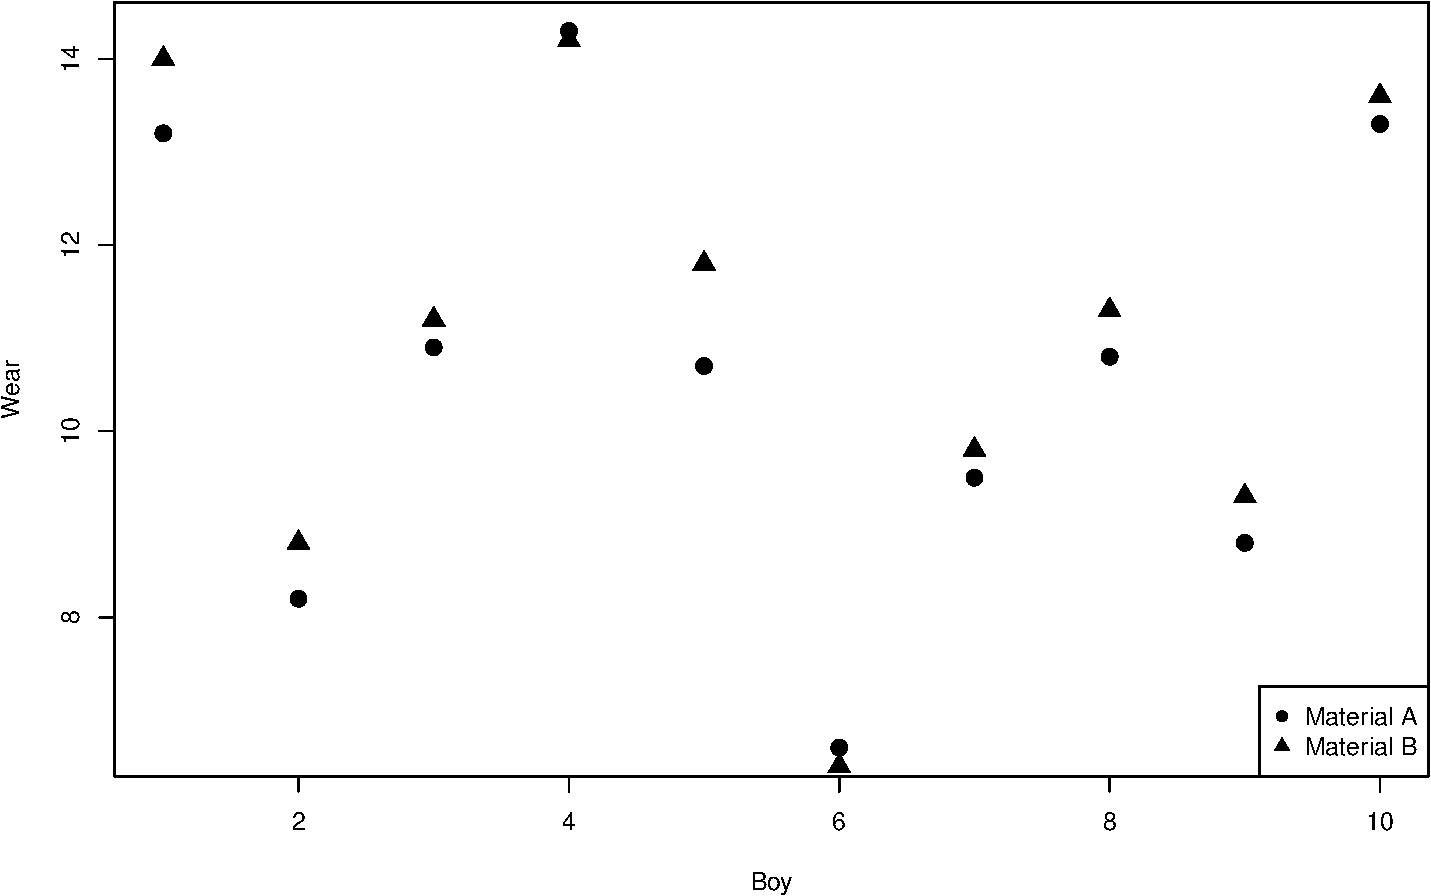
\includegraphics{class4slides-jan18_files/figure-beamer/unnamed-chunk-19-1.pdf}

\end{frame}

\begin{frame}[fragile]{Randomized paired comparison}

\begin{Shaded}
\begin{Highlighting}[]
\NormalTok{diff <-}\StringTok{ }\NormalTok{shoes.data$matA-shoes.data$matB}
\NormalTok{meandiff <-}\StringTok{ }\KeywordTok{mean}\NormalTok{(diff); meandiff}
\end{Highlighting}
\end{Shaded}

\begin{verbatim}
## [1] -0.41
\end{verbatim}

\begin{Shaded}
\begin{Highlighting}[]
\NormalTok{shoe.dat2 <-}\StringTok{ }\KeywordTok{data.frame}\NormalTok{(shoes.data,diff)}
\NormalTok{shoe.dat2}
\end{Highlighting}
\end{Shaded}

\begin{verbatim}
##    boy matA sideA matB sideB diff
## 1    1 13.2     L 14.0     R -0.8
## 2    2  8.2     L  8.8     R -0.6
## 3    3 10.9     R 11.2     L -0.3
## 4    4 14.3     L 14.2     R  0.1
## 5    5 10.7     R 11.8     L -1.1
## 6    6  6.6     L  6.4     R  0.2
## 7    7  9.5     L  9.8     R -0.3
## 8    8 10.8     L 11.3     R -0.5
## 9    9  8.8     R  9.3     L -0.5
## 10  10 13.3     L 13.6     R -0.3
\end{verbatim}

\end{frame}

\begin{frame}{Boy's Shoe Experiment}

\begin{itemize}
\item
  The sequence of coin tosses is one of \(2^{10}=1024\) equiprobable
  outcomes.
\item
  To test \(H_0\) the average difference of -0.41 observed observed can
  be compared with the other 1023 averages by calculating the average
  difference for each of 1024 arrangements of signs in:
\end{itemize}

\[{\bar d} = \frac{\pm 0.8 \pm0.6 \cdots \pm 0.3}{10}\]

\end{frame}

\begin{frame}[fragile]{Randomized paired comparison}

\begin{Shaded}
\begin{Highlighting}[]
\NormalTok{N <-}\StringTok{ }\DecValTok{2}\NormalTok{^(}\DecValTok{10}\NormalTok{) }\CommentTok{# number of treatment assignments}
\NormalTok{res <-}\StringTok{ }\KeywordTok{numeric}\NormalTok{(N) }\CommentTok{#vector to store results}
\NormalTok{LR <-}\StringTok{ }\KeywordTok{list}\NormalTok{(}\KeywordTok{c}\NormalTok{(-}\DecValTok{1}\NormalTok{,}\DecValTok{1}\NormalTok{)) }\CommentTok{# difference is multiplied by -1 or 1}
\CommentTok{# generate all possible treatment assign}
\NormalTok{trtassign <-}\StringTok{ }\KeywordTok{expand.grid}\NormalTok{(}\KeywordTok{rep}\NormalTok{(LR, }\DecValTok{10}\NormalTok{)) }

\NormalTok{for(i in }\DecValTok{1}\NormalTok{:N)\{}
\NormalTok{res[i] <-}\StringTok{ }\KeywordTok{mean}\NormalTok{(}\KeywordTok{as.numeric}\NormalTok{(trtassign[i,])*diff)}
\NormalTok{\}}
\NormalTok{trtassign[}\DecValTok{1}\NormalTok{:}\DecValTok{2}\NormalTok{,]}
\end{Highlighting}
\end{Shaded}

\begin{verbatim}
##   Var1 Var2 Var3 Var4 Var5 Var6 Var7 Var8 Var9 Var10
## 1   -1   -1   -1   -1   -1   -1   -1   -1   -1    -1
## 2    1   -1   -1   -1   -1   -1   -1   -1   -1    -1
\end{verbatim}

\begin{Shaded}
\begin{Highlighting}[]
\NormalTok{res[}\DecValTok{1}\NormalTok{:}\DecValTok{2}\NormalTok{]}
\end{Highlighting}
\end{Shaded}

\begin{verbatim}
## [1] 0.41 0.25
\end{verbatim}

\end{frame}

\begin{frame}[fragile]{Randomized paired comparison}

\begin{Shaded}
\begin{Highlighting}[]
\KeywordTok{hist}\NormalTok{(res, }\DataTypeTok{xlab=}\StringTok{"Mean Difference"}\NormalTok{,}\DataTypeTok{main=}\StringTok{"Randomization Distribution Boys' Shoes"}\NormalTok{)}
\KeywordTok{abline}\NormalTok{(}\DataTypeTok{v =} \NormalTok{meandiff,}\DataTypeTok{col=}\StringTok{"blue"}\NormalTok{)}
\end{Highlighting}
\end{Shaded}

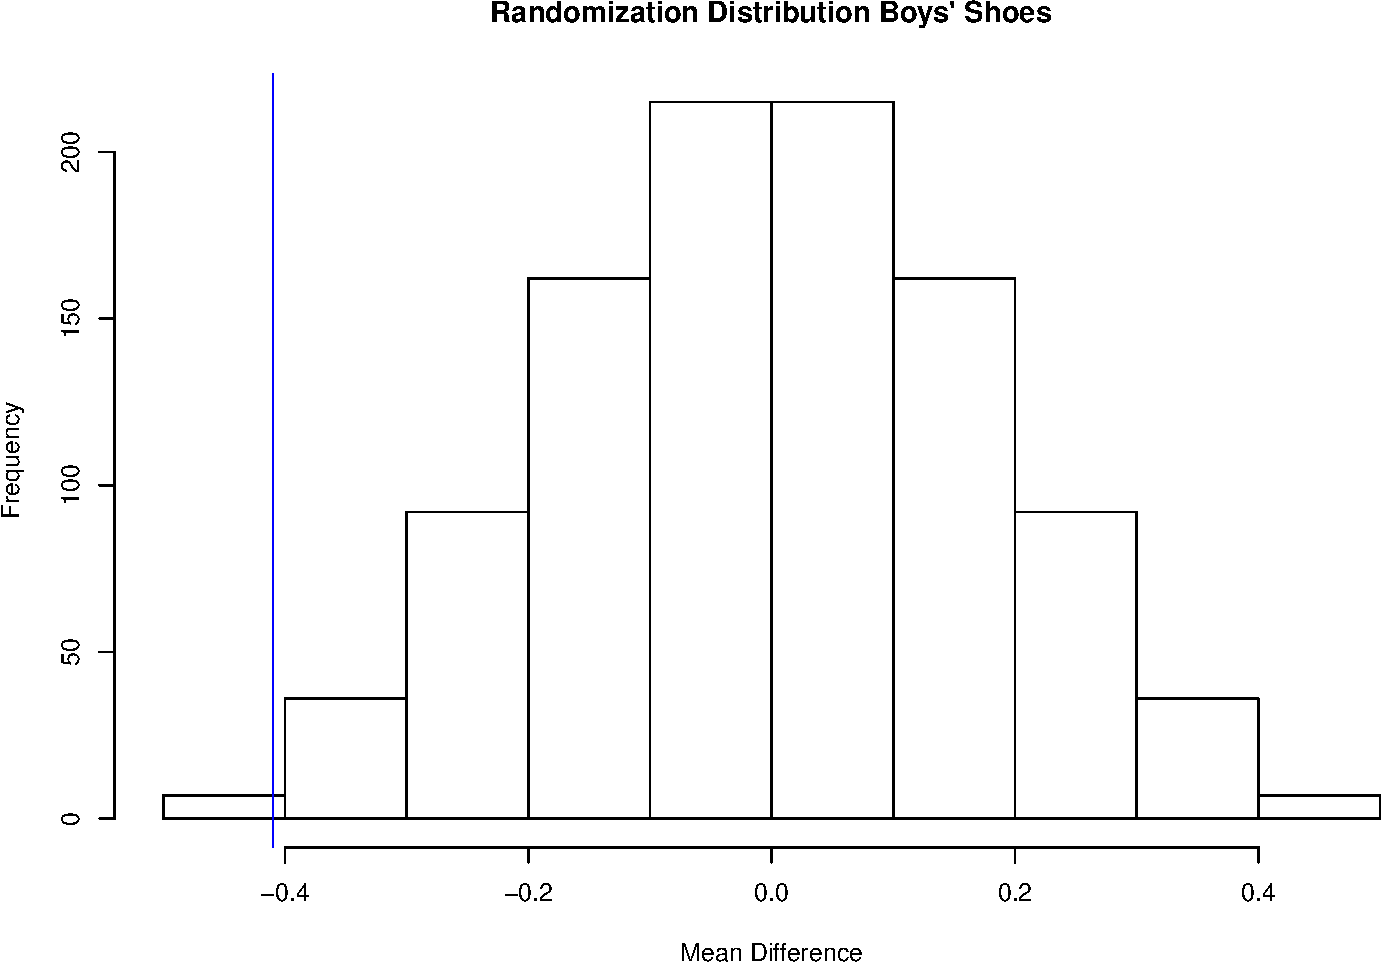
\includegraphics{class4slides-jan18_files/figure-beamer/unnamed-chunk-22-1.pdf}

\end{frame}

\begin{frame}[fragile]{Randomized paired comparison}

\begin{Shaded}
\begin{Highlighting}[]
\KeywordTok{sum}\NormalTok{(res<=meandiff) }\CommentTok{# number of differences le observed diff}
\end{Highlighting}
\end{Shaded}

\begin{verbatim}
## [1] 7
\end{verbatim}

\begin{Shaded}
\begin{Highlighting}[]
\KeywordTok{sum}\NormalTok{(res<=meandiff)/N }\CommentTok{# p-value}
\end{Highlighting}
\end{Shaded}

\begin{verbatim}
## [1] 0.006835938
\end{verbatim}

\end{frame}

\begin{frame}{Paired t-test}

If we assume that the differences -0.8, -0.6, -0.3, 0.1, -1.1, 0.2,
-0.3, -0.5, -0.5, -0.3 are a random sample from a normal distribution
then the statistic

\[t=\frac{{\bar d}}{s_{\bar d}/\sqrt{10}} \sim t_{10-1},\]

where, \(s_{\bar d}\) is the sample standard deviation of the paired
differences. The p-value for testing if \({\bar D} < 0\) is

\[ P(t_{9}< t).\]

\end{frame}

\begin{frame}{Paired t-test}

In general if there are \(n\) differences then

\[t=\frac{{\bar d}}{s_{\bar d}/\sqrt{n}} \sim t_{n-1},\]

where, \(s_{\bar d}\) is the sample standard deviation of the paired
differences. The p-value for testing if \({\bar D} < 0\) is

\[ P(t_{n-1}< t).\]

NB: This is the same as a one-sample t-test of the differences.

\end{frame}

\begin{frame}[fragile]{Paired t-test}

In R a paired t-test can be obtained by using the command
\texttt{t.test()} with \texttt{paired=T}.

\begin{Shaded}
\begin{Highlighting}[]
\KeywordTok{t.test}\NormalTok{(shoes.data$matA,shoes.data$matB,}\DataTypeTok{paired =} \OtherTok{TRUE}\NormalTok{,}
       \DataTypeTok{alternative =} \StringTok{"less"}\NormalTok{)}
\end{Highlighting}
\end{Shaded}

\begin{verbatim}
## 
##  Paired t-test
## 
## data:  shoes.data$matA and shoes.data$matB
## t = -3.3489, df = 9, p-value = 0.004269
## alternative hypothesis: true difference in means is less than 0
## 95 percent confidence interval:
##        -Inf -0.1855736
## sample estimates:
## mean of the differences 
##                   -0.41
\end{verbatim}

\end{frame}

\begin{frame}[fragile]{Paired t-test}

This is the same as a one-sample t-test on the difference.

\begin{Shaded}
\begin{Highlighting}[]
\CommentTok{# same as a one-sample t-test on the diff}
\KeywordTok{t.test}\NormalTok{(diff,}\DataTypeTok{alternative =} \StringTok{"less"}\NormalTok{) }
\end{Highlighting}
\end{Shaded}

\begin{verbatim}
## 
##  One Sample t-test
## 
## data:  diff
## t = -3.3489, df = 9, p-value = 0.004269
## alternative hypothesis: true mean is less than 0
## 95 percent confidence interval:
##        -Inf -0.1855736
## sample estimates:
## mean of x 
##     -0.41
\end{verbatim}

\end{frame}

\begin{frame}[fragile]{Paired t-test}

\begin{Shaded}
\begin{Highlighting}[]
\KeywordTok{qqnorm}\NormalTok{(diff); }\KeywordTok{qqline}\NormalTok{(diff)}
\end{Highlighting}
\end{Shaded}

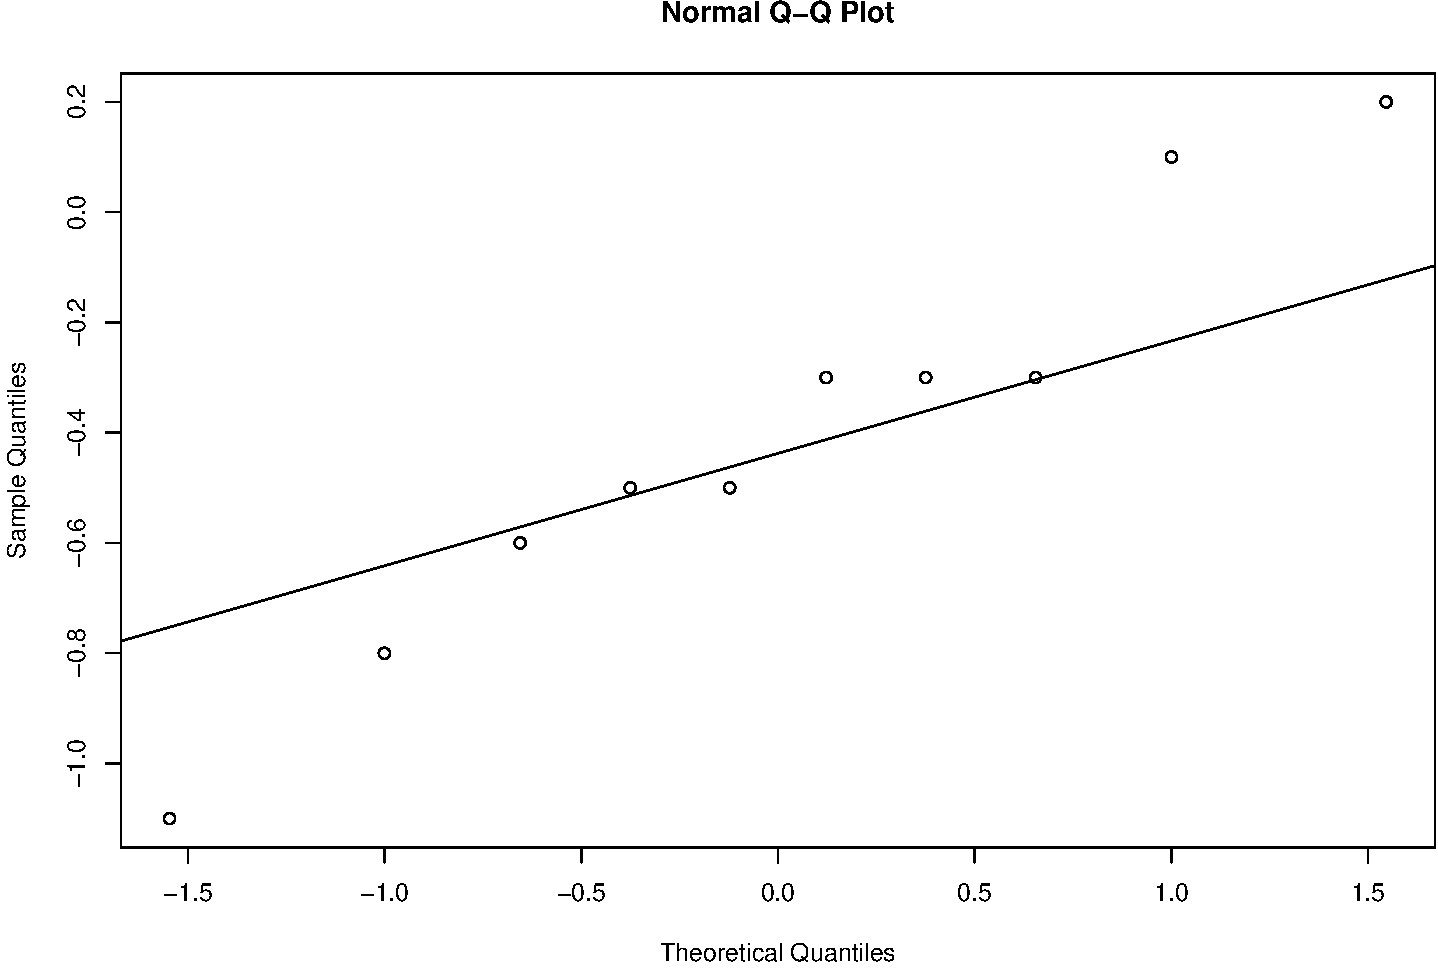
\includegraphics{class4slides-jan18_files/figure-beamer/unnamed-chunk-26-1.pdf}

\end{frame}

\end{document}
